%% abtex2-modelo-slides.tex, v-1.0 gfabinhomat
%% Copyright 2012-2018 by abnTeX2 group at http://www.abntex.net.br/ 
%%
%% This work may be distributed and/or modified under the
%% conditions of the LaTeX Project Public License, either version 1.3
%% of this license or (at your option) any later version.
%% The latest version of this license is in
%%   http://www.latex-project.org/lppl.txt
%% and version 1.3 or later is part of all distributions of LaTeX
%% version 2005/12/01 or later.
%%
%% This work has the LPPL maintenance status `maintained'.
%% 
%% The Current Maintainer of this work is Fábio Rodrigues Silva, 
%% member of abnTeX2 team, led by Lauro César Araujo. 
%% Further information are available on 
%% http://www.abntex.net.br/
%%
%% This work consists of the files abntex2-modelo-slides.tex, 
%% abntex2-modelo-references.bib and abntex2-modelo-marca.pdf
%%
%% Modelo desenvolvido por Fábio Rodrigues Silva (gfabinhomat@gmail.com)
%% Mais informações podem ser obtidas no guia do usuário Beamer 
%% (http://linorg.usp.br/CTAN/macros/latex/contrib/beamer/doc/beameruserguide.pdf)
%% Informações rápidas podem ser acessadas em http://en.wikibooks.org/wiki/LaTeX/Presentations


% Apresentações em widescreen. Outros valores possíveis: 1610, 149, 54, 43 e 32.
% Por padrão, as apresentações são no formato 4:3 (sem o aspectratio).
\documentclass[aspectratio=169]{beamer}	 	

% ---
% PACOTES
% ---
\usepackage[alf]{abntex2cite}		% Citações padrão ABNT
\usepackage[brazil]{babel}		% Idioma do documento
\usepackage{color}			% Controle das cores
\usepackage[T1]{fontenc}		% Selecao de codigos de fonte.
\usepackage{graphicx}			% Inclusão de gráficos
\usepackage[utf8]{inputenc}		% Codificacao do documento (conversão automática dos acentos)
\usepackage{txfonts}			% Fontes virtuais
\usepackage{datetime}

% ---

% \usetheme{Pittsburgh}
\usetheme{Frankfurt}
\usecolortheme{default}
\usefonttheme[onlymath]{serif}			% para fontes matemáticas
% Enconte mais temas e cores em http://www.hartwork.org/beamer-theme-matrix/ 
% Veja também http://deic.uab.es/~iblanes/beamer_gallery/index.html



\newdateformat{monthyeardate}{%
  \monthname[\THEMONTH], \THEYEAR}

\definecolor{light-gray}{gray}{0.95}
\definecolor{dark-blue}{rgb}{.18, .19, .58}


% Configuração footline
\setbeamertemplate{navigation symbols}{}
\setbeamertemplate{footline}
{
  \leavevmode%
  \hbox{%
  \begin{beamercolorbox}[wd=.333333\paperwidth,ht=2.25ex,dp=1ex,center]{section in head/foot}%
    \usebeamerfont{author in head/foot}\insertshortauthor
  \end{beamercolorbox}%
  \begin{beamercolorbox}[wd=.333333\paperwidth,ht=2.25ex,dp=1ex,center]{section in head/foot}%
    \usebeamerfont{title in head/foot}Trabalho de Conclusão de Curso I
  \end{beamercolorbox}%
  \begin{beamercolorbox}[wd=.333333\paperwidth,ht=2.25ex,dp=1ex,right]{section in head/foot}%
    \usebeamerfont{date in head/foot}Novembro, 2019\hspace*{2em}
    \insertframenumber{} / \inserttotalframenumber\hspace*{2ex} 
  \end{beamercolorbox}}%
  \vskip0pt%
}

% Customizações de Cores: fg significa cor do texto e bg é cor do fundo
\setbeamercolor{normal text}{fg=black}
\setbeamercolor{alerted text}{fg=red}
\setbeamercolor{author}{fg=black}
\setbeamercolor{institute}{fg=black}
\setbeamercolor{date}{fg=blue}
\setbeamercolor{frametitle}{fg=white}
\setbeamercolor{framesubtitle}{fg=white}
\setbeamercolor{block title}{bg=dark-blue, fg=white}		%Cor do título
\setbeamercolor{block body}{bg=light-gray, fg=black}	%Cor do texto (bg= fundo; fg=texto)



% --- Informações do documento ---
\title{Desenvolvimento de uma Inteligência Artificial para aprender a jogar jogos em Allegro}
% \subtitle{TCC}
\author{Arthur de Senna Rocha}
\institute{}

\institute[VFU] % (optional)
{
  % \inst{1}%
  	Universidade Federal de Minas Gerais
	\par
	Escola de Engenharia
  \and
  % \inst{2}%
  Trabalho de Conclusão de Curso I
}

\date{\today}
% \shortdate{}
% ---

% ----------------- INÍCIO DO DOCUMENTO --------------------------------------
\begin{document}

% ----------------- NOVO SLIDE --------------------------------
\begin{frame}

% \begin{minipage}{1\linewidth}
%   \centering
%   \begin{tabular}{cc}
%     \begin{tabular}{c}
%       
\includegraphics[width=3.0cm]{aplicacoes_ufmg/principal_ufmg.jpg}
%     \end{tabular}
%     &
%     \begin{tabular}{c}
%       \textbf{Universidade Federal de Minas Gerais} \\ \textbf{Escola de Engenharia}
%     \end{tabular}
%   \end{tabular}
% \end{minipage}

\titlepage

\end{frame}

% ----------------- NOVO SLIDE --------------------------------
\begin{frame}{Sumário}
\tableofcontents
\end{frame}

% ----------------- NOVO SLIDE --------------------------------
\section{Introdução}
\stepcounter{subsection}
\begin{frame}{Introdução}

\begin{block}{\large{{Proposta}}}
	\begin{itemize}
		\item Desenvolver uma IA capaz de aprender a jogar diferentes jogos;
		\item Algoritmo de Deep Reinforcement Learning;
		\item Nenhuma regra sobre o jogo é dada e, inicialmente, a IA não tem informações sobre o que precisa fazer.
		% \item A única informação passada para a IA são os comandos básicos do jogo;
		% \item Acesso ao código fonte dos jogos;
		% \item Jogos devem feito em Allegro.
	\end{itemize}
\end{block}

% O uso de inteligência artificial (IA) e de algoritmos de machine learning possibilita que máquinas aprendam com experiências, se ajustem à novas entradas de dados e performem tarefas como seres humanos. Com essas tecnologias, os computadores podem ser treinados para cumprir tarefas específicas ao processar grandes quantidades de dados e reconhecer padrões nesses dados. O presente trabalho se propõe a desenvolver uma IA capaz de aprender a jogar diferentes jogos, desde que se tenha acesso ao código fonte e feito em Allegro. Para isso, será implementado um algoritmo de Deep Reinforcement Learning, abordagem que consiste em fornecer ao sistema parâmetros relacionados ao seu estado e uma recompensa positiva ou negativa com base em suas ações. Nenhuma regra sobre o jogo é dada e, inicialmente, a IA não tem informações sobre o que precisa fazer. A única informação passada para a IA são os comandos básicos do jogo. O objetivo do sistema é descobrir e elaborar uma estratégia para maximizar a pontuação - ou a recompensa. Diferente de muitas IAs que focam na solução de um único problema, a proposta deste projeto é elaborar uma IA que seja genérica e capaz solucionar e elaborar estratégias para uma variedade de situações diferentes.

\end{frame}

\begin{frame}{Motivação}

\begin{block}{\large{{Aprendizado de máquina}}}
	\begin{itemize}
		% \item Técnicas de ML e algoritmos de DL têm consistentemente melhorado a capacidade de um computador de fornecer reconhecimento de padrões e previsões cada vez mais precisas;
		\item Sistemas de DL são consistentemente aplicados com sucesso a conjuntos de aplicações cada vez mais amplos;
		\item A complexidade das tarefas que podem ser resolvidas por DL vêm crescendo significativamente;
		\item Valor para pesquisa em múltiplas áreas da ciência;
		\item Aplicações de aprendizado de máquina e deep learning são altamente lucrativas;
		\item Potencial de investimento em pesquisa, modelagem de novos problemas e estudo de técnicas de aprendizado de máquina.
	\end{itemize}
\end{block}

\end{frame}
\begin{frame}{Motivação}

\begin{block}{\large{{DL em Jogos Digitais}}}
	\begin{itemize}
		\item Indústria de jogos digitais tem testemunhado um enorme crescimento nos últimos anos;
		\item IA e DL são utilizados em inúmeras aplicações em diversos jogos;
		\item Fornecer uma melhor experiência para o usuário;
		\item Potencial dessas ferramentas de obter uma vantagem competitiva no mercado.
	\end{itemize}
\end{block}

\end{frame}

\begin{frame}{Descrição do Problema}
	\begin{block}{\large{{O Agente}}}
		\begin{itemize}
			\item O sistema receberá, inicialmente, somente as limitações físicas do jogo;

			\item O agente deve ser capaz de elaborar uma estratégia para maximizar sua pontuação;

			\item O sistema deverá ser capaz de lidar com cenários aleatórios e não-aleatórios;

			\item O sistema deve ser generalizado para que possa ser aplicado à diferentes cenários e treinado para jogar diferentes jogos.
			% \item Acesso ao código fonte dos jogos;
			% \item Jogos devem feito em Allegro.
		\end{itemize}
	\end{block}
	\pause
	\begin{block}{\large{{Restrições}}}
		\begin{itemize}
			\item Acesso ao código fonte dos jogos;
			\item Jogos devem ser implementados em \textit{Allegro};
			\item Jogos devem ser 2D.
		\end{itemize}
	\end{block}

\end{frame}

\begin{frame}{Descrição do Problema}
	
	\begin{block}{\large{{Objetivos}}}
		\begin{itemize}
			\item Criar e treinar uma rede neural convolucional capaz de aprender políticas através de pixels brutos em ambientes complexos;

			\item O agente deve alcançar resultados superiores aos de uma abordagem aleatória e próximos aos de um agente humano;

			\item Implementar um agente que seja capaz de aprender a jogar o maior número de jogos possíveis sem conhecimento prévio do ambiente.
		\end{itemize}
	\end{block}
\end{frame}

% ----------------- Nova Seção --------------------------------
\section{Contextualização em Humanidades}
\stepcounter{subsection}
\begin{frame}{Contextualização em Humanidades}

	\begin{figure}[h]
	  \centering
	  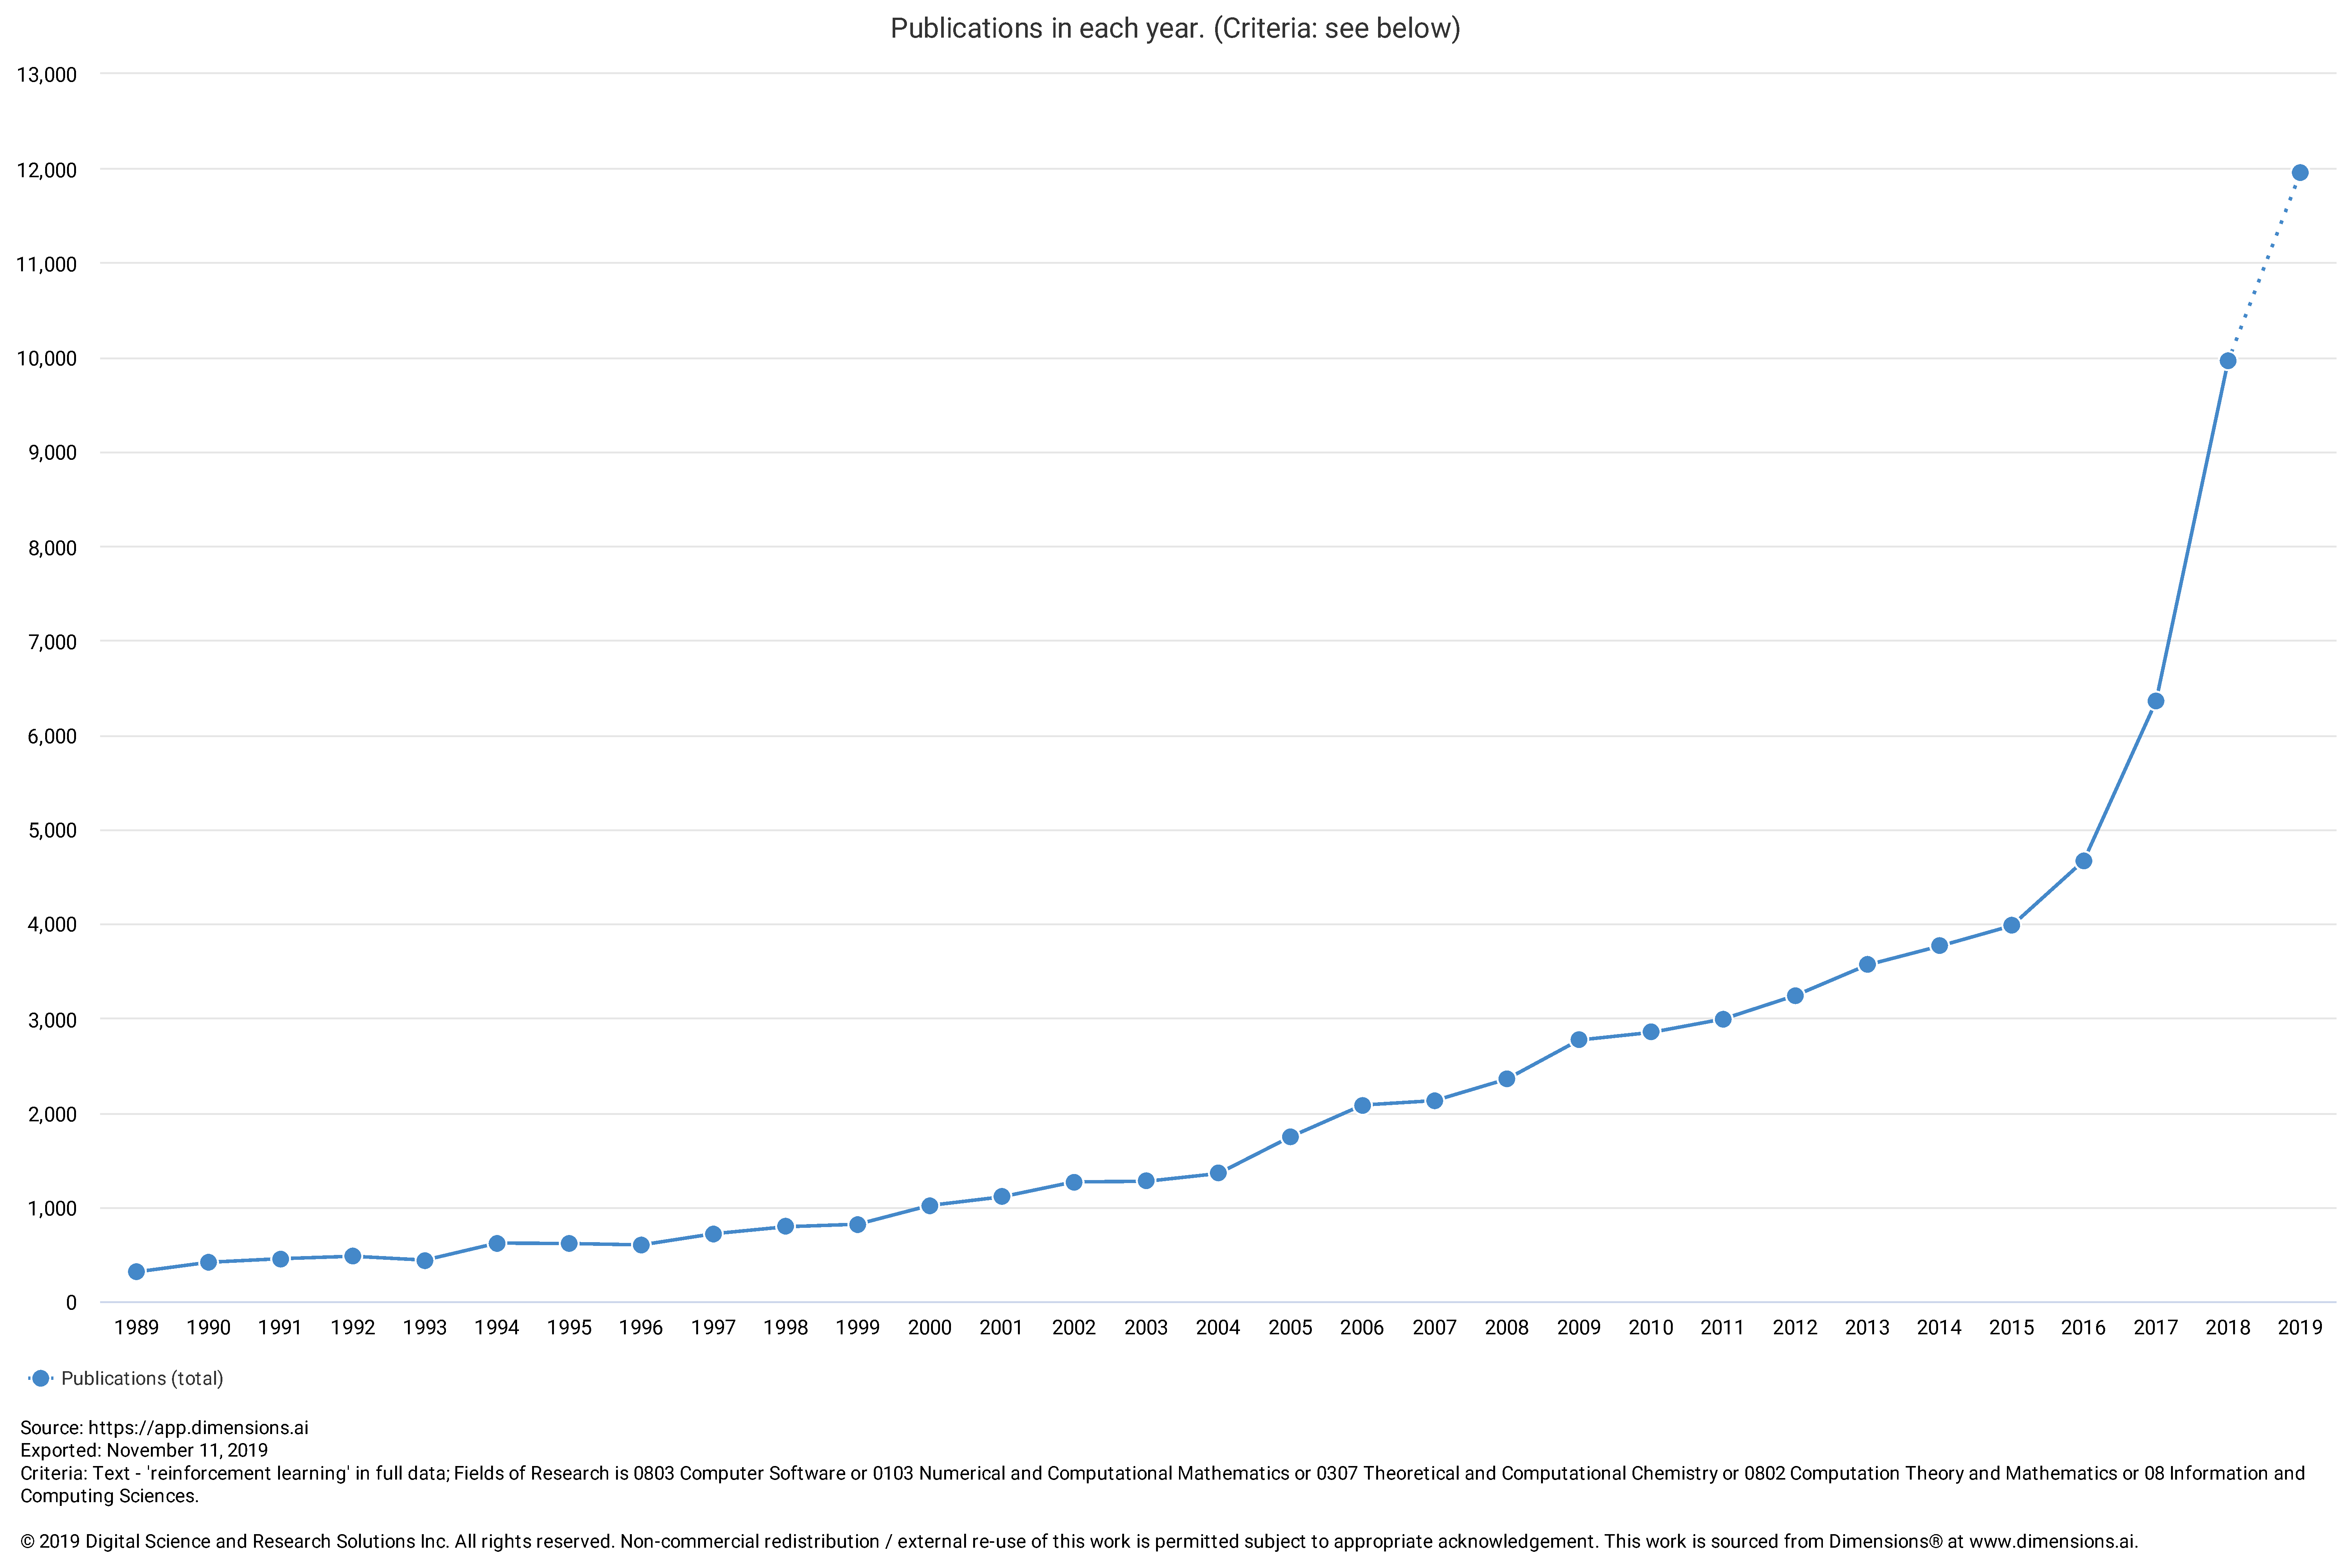
\includegraphics[width=.7 \textwidth]{imgs/rl-publications-overview.pdf}
	  % \caption{}
	  \label{publications-overview}
	 \end{figure}
\end{frame}

\begin{frame}{Aplicações de \textit{Deep Learning}}
	\begin{block}{Análise social}
		\begin{itemize}
			\item Reconhecimento de fala \cite{nassif:speech-rec:2019};
			\item Modelos de processamento visual com diversas aplicações na medicina \cite{Yeung:comp-vis:2019};
			\item Utilização para estimar as características socioeconômicas de diferentes regiões a partir de imagens de cenas de rua reunidas com carros do \textit{Google Street View} \cite{Gebru13108};
			\item Predição interação entre moléculas, a fim de ajudar as empresas farmacêuticas a projetar novos medicamentos \cite{dahl2014multitask}.
		\end{itemize}
	\end{block}
\end{frame}

\begin{frame}{Aplicações de \textit{Deep Learning}}
	\begin{block}{Análise Econômica}
		\begin{itemize}
			\item Ferramentas que melhoram a precisão dos sensores de precipitação por satélite e concentrando-se na redução do viés e dos alarmes falsos \cite{doi:10.1175/JHM-D-15-0075.1};
			\item Agentes que permitem que diferentes dispositivos eletrônicos interpretem dados de multimídia não estruturados e reajam de maneira inteligente aos eventos do usuário e do ambiente \cite{dl-IoT};
			\item Grandes empresas como o \textit{Google, Amazon} e \textit{Netflix} utilizam ferramentas de \textit{deep learning} como peça essencial em seus produtos.
		\end{itemize}
	\end{block}
\end{frame}
\begin{frame}{Aplicações de \textit{Deep Learning}}
	\begin{block}{Inteligência Artificial em Jogos}
		\begin{itemize}
			% \item ;
			\item Ajudar na jogabilidade;
			\item Melhorar a imersão do jogador no mundo do jogo;
			\item Simular a psicologia dos agentes NPC;
			\item Apoiar o trabalho de designers de jogos e níveis \cite{Piergigli:drl:2019};
			\item Treinar um agente para superar os jogadores humanos e otimizar sua pontuação pode nos ensinar como otimizar diferentes processos em diversas situações.
		\end{itemize}
	\end{block}
\end{frame}
% ----------------- Nova Seção --------------------------------
\section{Abordagem Proposta}
\stepcounter{subsection}

\begin{frame}{Abordagem Proposta}
	\begin{block}{\textit{Deep Learning}}
		\begin{itemize}
			\item Área do aprendizado de máquina que propõe que os computadores aprendam com a experiência;
			\item Ajustem à novas entradas de dados;
			\item Compreendam o mundo em termos de hierarquia de conceitos, sendo cada conceito definido por sua relação com conceitos mais simples.
		\end{itemize}
	\end{block}
\end{frame}

\begin{frame}{\textit{Deep Learning}}
	\begin{figure}[h]
	  \centering
	  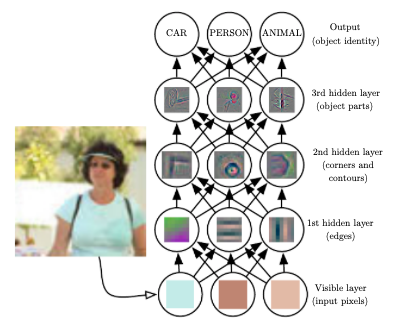
\includegraphics[width=.5 \textwidth]{imgs/hierarquia-conceitos-dl.png}
	  % \caption{}
	  \label{hierarquia-conceitos}
	 \end{figure}
\end{frame}

% \begin{frame}{Rede Neural}

% \begin{tabular}{lc}  
% 		\begin{tabular}{l}
%              \parbox{0.4\linewidth}{%  change the parbox width as appropiate
%             	  \begin{itemize}
%             	  	\item Rede neural composta de múltiplas camadas;
%             	  	\item Cada neurônio é caracterizado pelo um \textbf{peso}, \textbf{bias} e uma \textbf{função de ativação};
%             	  	\item A informação se move da camada de entrada para as camadas ocultas;

%             	  \end{itemize}
% 		    }
% 	    \end{tabular} & 

%          \begin{tabular}{c}
%            \hspace{-.6cm}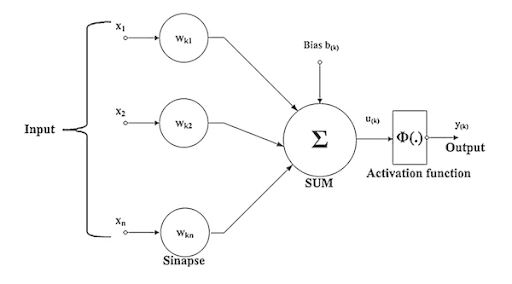
\includegraphics[width=.6 \textwidth]{imgs/neuronio.png}
%            \end{tabular}
           
           
% 	\end{tabular}
	
% \end{frame}

% \begin{frame}{Rede Neural}

% \begin{tabular}{lc}  
% 		\begin{tabular}{l}
%              \parbox{0.4\linewidth}{%  change the parbox width as appropiate
%             	  \begin{itemize}
%             	  	\item As camadas ocultas fazem o processamento e enviam a saída final para a camada de saída;
%             	  	\item Os pesos e bias dos neurônios são atualizados com base no erro;
%             	  	\item Uma vez que todos os dados passaram por este processo, os pesos e bias finais são usados para previsões;

%             	  \end{itemize}
% 		    }
% 	    \end{tabular} & 

%          \begin{tabular}{c}
%            \hspace{-.6cm}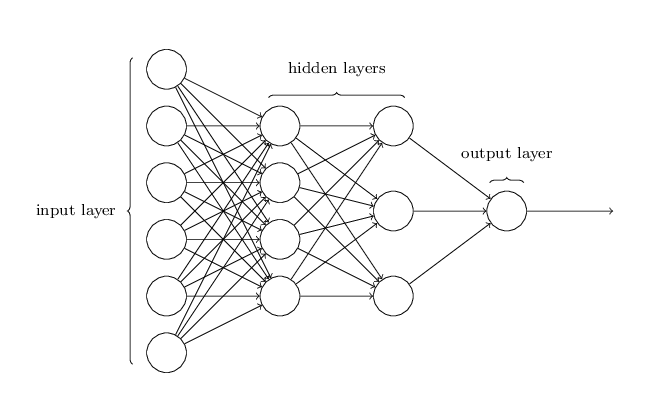
\includegraphics[width=.6 \textwidth]{imgs/deep-neural-network.png}
%            \end{tabular}
           
           
% 	\end{tabular}
	
% \end{frame}

\begin{frame}{Abordagem Proposta}
	\begin{block}{\textit{Reinforcement Learning}}
		\begin{itemize}
			\item Abordagem computacional para entender e automatizar o aprendizado direcionado a objetivos e a tomada de decisões;
			\item Ênfase na aprendizagem de um agente apartir da interação direta com seu ambiente, em exigir supervisão exemplar ou modelos completos do ambiente;
			\item Abordagem caracterizada por tentativa e erro e recompensa atrasada.
		\end{itemize}
	\end{block}
	% \begin{figure}[h]
	%   \centering
	%   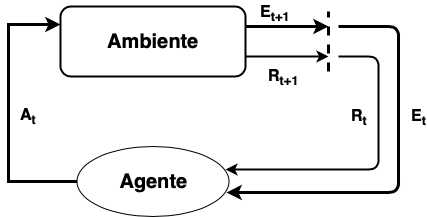
\includegraphics[width=.4 \textwidth]{imgs/rl-diagram.png}
	%   % \caption{}
	%   \label{rl-diagram}
	%  \end{figure}
\end{frame}



\begin{frame}{\textit{Reinforcement Learning}}

\begin{tabular}{lc}  
		\begin{tabular}{l}
             \parbox{0.5\linewidth}{%  change the parbox width as appropiate
            	  \begin{itemize}
            	  	\item A \textbf{política} define a maneira que o agente deve se comportar em um determinado momento;
            	  	\item Um \textbf{sinal de recompensa} define o objetivo de um problema de aprendizado por reforço;
            	  	\item A \textbf{função de valor} especifica o que é bom a longo prazo;
            	  	\item Objetivo final é maximizar a função de valor

            	  \end{itemize}
		    }
	    \end{tabular} & 

         \begin{tabular}{c}
           \hspace{-.5cm}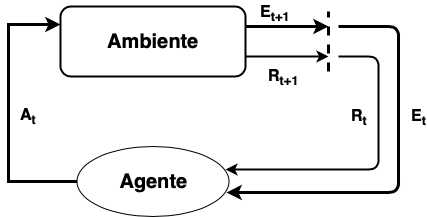
\includegraphics[width=.5 \textwidth]{imgs/rl-diagram.png}
           \end{tabular}
           
           
	\end{tabular}
	
\end{frame}

\begin{frame}{Abordagem Proposta}
	\begin{block}{\textit{Deep Reinforcement Learning}}
		\begin{itemize}
			\item 
			O \textit{deep reinforcement learning} (DRL) é uma abordagem do \textit{deep learning} que, em contraste a abordagens mais tradicionais como o aprendizado supervisionado e não supervisionado, utiliza as técnicas de aprendizagem por reforço para treinar o agente;

			\item Essa abordagem consiste em fornecer ao sistema parâmetros relacionados ao seu estado e uma recompensa positiva ou negativa com base em suas ações.
		\end{itemize}
	\end{block}
\end{frame}

\begin{frame}{Abordagem Proposta}
	\begin{block}{\textit{Allegro Learning Enviroment}}
		\begin{itemize}
			\item Inspirado no \textit{Arcade Learning Enviroment}, uma ferramenta de software que oferece uma interface para interagir com ambientes de jogos Atari 2600 emulados;

			\item Objetivo de oferecer uma plataforma que facilite o desenvolvimento de agentes de aprendizado para jogos Atari;

			\item O \textit{Allegro Learning Enviroment} funcionaria de forma semelhante e teria como base a ferramenta implementada por \cite{silva:amb-jd-allegro};

			\item Ferramenta fornece funcionalidades como a exportação dos comandos básicos de um jogo feito em \textit{Allegro} e capturas de tela;

			\item Permite que o pesquisador não fique limitado a um jogo existente, mas possa usar qualquer jogo que ele tenha acesso ao código fonte e feito em \textit{Allegro}.
		\end{itemize}
	\end{block}
\end{frame}

\begin{frame}{Abordagem Proposta}
	\begin{block}{Treinamento}
		\begin{itemize}
			\item Para o treinamento do agente, serão utilizados capturas da tela em cada estado do jogo, obtidas pelo ALE;
			\item A partir dessas imagens serão extraídas as informações do estado atual do jogo (posição do jogador, obstáculos, etc);
			\item A utilização de capturas de tela como entradas para o agente permite que a IA seja treinada para situações em que hajam obstáculos gerados de forma aleatória;
			\item A partir dessas imagens, o agente deverá ser capaz de identificar tais obstáculos, sua localização em relação ao jogador e a melhor maneira de lidar com os mesmos.
		\end{itemize}
	\end{block}
	
\end{frame}
\begin{frame}{Abordagem Proposta}
	\begin{block}{Os Jogos}
		\begin{itemize}
			\item Os jogos serão obtidos de fontes de código aberto disponíveis online;
			\item Caso seja necessário, serão implementados com os requisitos necessários para o projeto;
			\item A proposta é de se utilizar diferentes jogos de diferentes complexidades para avaliar o potencial do sistema.
		\end{itemize}
	\end{block}
\end{frame}

% ----------------- Nova Seção --------------------------------
\section{Considerações Finais}
\stepcounter{subsection}

\begin{frame}{Conclusões}
	\begin{block}{}
		\begin{itemize}
			\item A inteligência artificial e o aprendizado de máquina possuem inúmeras aplicações práticas;
			\item Treinar um agente em jogos digitais para superar os jogadores humanos e otimizar sua pontuação pode nos ensinar como otimizar processos variados com múltiplas aplicações;
			\item Com isso em mente, propõe-se implementar uma IA que seja capaz de aprender e desenvolver estratégias para jogar diferentes jogos;
			\item Utilizando técnicas de DRL existentes, espera-se produzir uma IA que seja flexível e que possa ser adaptada para diferentes cenários.
		\end{itemize}
	\end{block}
\end{frame}

\begin{frame}{Propostas de Continuidade}
	\begin{block}{}
		\begin{itemize}
			\item Modelagem matemática do problema;
			\item Descrição do algoritmo e decisões de implementação da ferramenta proposta;
			\item Implementação (se necessário) de diferentes jogos em Allegro para a validação do sistema;
			\item Implementação da rede neural e treinamento do agente em múltiplos jogos de diferentes complexidades;
			\item Análise crítica dos resultados obtidos.
		\end{itemize}
	\end{block}
\end{frame}

% ----------------- NOVO SLIDE --------------------------------
% \section{Fontes a serem consultadas}
% \stepcounter{subsection}
% \begin{frame}
% \frametitle{Público-Alvo}
% \framesubtitle{Usuários já iniciados ao Beamer}

% \begin{block}{Título}
%  Este modelo foi preparado como uma aplicação do uso do pacote abnTeX2 com o Beamer.
% \end{block}

% \begin{itemize}
%  \item Alguns comandos são explicados no modelo TEX. \pause
 
%  \item Para maiores informações, consulte o guia do usuário Beamer 
%  (\url{https://www.ctan.org/pkg/beamer})\pause
 
%  \item Para alterar o tema e as cores, consulte 
%  \url{http://deic.uab.es/~iblanes/beamer_gallery/index.html}
 
%  \item Consulte também \url{http://www.hartwork.org/beamer-theme-matrix/}
% \end{itemize}

% \end{frame}
% % % % ----------------- NOVO SLIDE --------------------------------
% % % \begin{frame}

% % % \begin{figure}
% % %   \centering
% % %   
\includegraphics[scale=1.0]{abntex2-modelo-img-marca.pdf}
% % %   \caption{Marca abnTeX2. Fonte: \url{http://www.abntex.net.br/}}
% % % \end{figure}

% % % \end{frame}

% % % % ----------------- NOVO SLIDE --------------------------------
% % % \begin{frame}{Participe dos grupos de discussão}

% % % \begin{itemize}
% % %   \item Tire dúvidas e ajude outros por meio do grupo de usuários LaTeX
% % %   \url{https://groups.google.com/group/latex-br} (e-mail:
% % %   \url{latex-br@googlegroups.com})
  
% % %   \item Proponha melhorias, avise sobre falhas e faça sugestões sobre o abnTeX2
% % %   no grupo dos desenvolvedores \url{https://groups.google.com/group/abntex2}
% % %   (e-mail: \url{abntex2@googlegroups.com});
% % % \end{itemize}

% % % Participe também da comunidade abnTeX2 no Google Plus
% % % \url{https://plus.google.com/u/0/communities/105202176004387477100}.

% % % \end{frame}

% % % ----------------- NOVO SLIDE --------------------------------
% % \section{Resultados}

% % \begin{frame}
% % \frametitle{ABNT}
% % \framesubtitle{Normas para trabalhos acadêmicos}

% % Para adequar seus documentos acadêmicos com as normas ABNT, utilize:
% % \begin{enumerate}
% %  \item \citeonline{NBR14724:2011}: Esta Norma especifica os princípios gerais
% %  para a elaboração de trabalhos acadêmicos (teses, dissertações e outros),
% %  visando sua apresentação à instituição (banca, comissão examinadora de
% %  professores, especialistas designados e/ou outros).
 
% %  \item \citeonline{NBR6028:2003}: Esta Norma estabelece os requisitos para
% %  redação e apresentação de resumos.
 
% %  \item \citeonline{NBR6024:2012}: Esta Norma especifica os princípios gerais
% %  para de um sistema de numeração progressiva das seções de um documento, de
% %  modo a expor numa seqüência lógica o inter-relacionamento da matéria e a
% %  permitir sua localização.
 
% %  \item \citeonline{NBR10520:2002}: Esta Norma especifica as características
% %  exigíveis para a apresentação de citações em documentos.
% % \end{enumerate}

% \end{frame}

% % ----------------- NOVO SLIDE --------------------------------
% \begin{frame}
% \frametitle{abnTeX2}
% \framesubtitle{Usando a suíte abnTeX2}

% Consulte \citeonline{abntex2-wiki-como-customizar} para customizações do abnTeX2.
% \vspace{0.5cm}

% Os documentos \citeonline{abntex2modelo-artigo},
% \citeonline{abntex2modelo-relatorio} e \citeonline{abntex2modelo} tratam dos
% principais trabalhos acadêmicos e suas aplicações ao TeX.
% \vspace{0.5cm}

% Para orientações sobre as citações e as referências com o abnTeX2, consulte
% \citeonline{abntex2cite} e \citeonline{abntex2cite-alf}.
% \vspace{0.5cm}

% \end{frame}

% ----------------- NOVO SLIDE --------------------------------
\section{Referências}
\stepcounter{subsection}

% --- O comando \allowframebreaks ---
% Se o conteúdo não se encaixa em um quadro, a opção allowframebreaks instrui 
% beamer para quebrá-lo automaticamente entre dois ou mais quadros,
% mantendo o frametitle do primeiro quadro (dado como argumento) e acrescentando 
% um número romano ou algo parecido na continuação.

\begin{frame}[allowframebreaks]{Referências}
\bibliography{referencias}
\end{frame}

% ----------------- FIM DO DOCUMENTO -----------------------------------------
\end{document}
